\documentclass{article}

\usepackage[final]{neurips_2025}

\usepackage[utf8]{inputenc}
\usepackage{CJKutf8}
\newcommand{\zh}[1]{\begin{CJK}{UTF8}{gbsn}#1\end{CJK}}
\newcommand{\ja}[1]{\begin{CJK}{UTF8}{min}#1\end{CJK}}
\usepackage[T1]{fontenc}
\usepackage{hyperref}
\usepackage{url}
\usepackage{booktabs}
\usepackage{amsfonts}
\usepackage{amsmath}
\usepackage{amssymb}
\usepackage{nicefrac}
\usepackage{subcaption}
\usepackage{microtype}
\usepackage{xcolor}
\usepackage{graphicx}
\usepackage{algorithm}
\usepackage{algorithmic}

\title{Embedding Inversion via Conditional Masked Diffusion Language Models}

\makeatletter
\renewcommand{\@noticestring}{Last updated: \today}
\makeatother

\author{%
  Han Xiao \\
  Jina AI by Elastic \\
  \texttt{han.xiao@jina.ai} \\
}

\begin{document}

\maketitle

\begin{abstract}
We frame embedding inversion as conditional masked diffusion, recovering all tokens in parallel through iterative denoising rather than sequential autoregressive generation. A masked diffusion language model is conditioned on the target embedding via adaptive layer normalization, requiring only 8 forward passes through a 78M parameter model with no access to the target encoder. On 32-token sequences across three embedding models, the method achieves 81.3\% token accuracy and 0.87 cosine similarity. Source code and live demo are available at \url{https://github.com/hanxiao/embedding-inversion-demo}.
\end{abstract}

\section{Introduction}

Text embeddings power modern retrieval systems, and production deployments routinely treat them as safe, anonymized representations. Vec2Text~\citep{morris2023text} challenged this assumption by recovering 92\% of 32-token sequences from their embeddings using a T5 encoder-decoder with iterative correction. Subsequent work has expanded the attack surface: ALGEN~\citep{algen} enables cross model inversion with few-shot alignment, and Zero2Text~\citep{zero2text} achieves training free inversion via LLM priors and online regression.

These methods share a common design: they generate tokens autoregressively, then iteratively re-embed the hypothesis to compute a correction signal. This creates two practical bottlenecks. First, each correction step requires a forward pass through the target embedding model, making the attack cost proportional to the number of iterations. Vec2Text typically requires over 20 iterations per sequence. Second, the autoregressive backbone accumulates errors left-to-right, with no mechanism to revise earlier tokens based on later context.

We propose an alternative formulation: embedding inversion as \textit{conditional masked diffusion}. Starting from a fully masked sequence, a denoising model iteratively reveals tokens at all positions in parallel, conditioned on the target embedding vector via adaptive layer normalization. The key structural difference is that correction is built into the diffusion process itself: each denoising step refines all positions simultaneously using global context, without ever reembedding the current hypothesis. This eliminates the need for access to the target encoder at inference time and reduces attack cost to a fixed number of forward passes through a small model of 78M parameters.

The approach is encoder agnostic by construction. The embedding vector enters only through AdaLN modulation of layer normalization parameters, so the same architecture and training procedure applies to any embedding model without alignment training or architecture specific modifications. We demonstrate this by training on three different encoders: jina-embeddings-v3 with 1024 dimensions, Qwen3-Embedding-0.6B with 1024 dimensions, and EmbeddingGemma-300m with 768 dimensions.

\begin{figure}[t]
\centering
\includegraphics[width=\textwidth]{figures/architecture.png}
\caption{Architecture of the Conditional Masked Diffusion Language Model. The embedding vector is projected and injected into each transformer layer via AdaLN conditioning. The model predicts original tokens at masked positions through iterative denoising.}
\label{fig:architecture}
\end{figure}

We present the first application of masked diffusion language models to embedding inversion, replacing autoregressive generation and iterative reembedding with parallel denoising. The approach is encoder agnostic: we train on three embedding models without alignment training or architecture specific modifications. We systematically compare four decoding strategies, identifying adaptive remasking during Euler sampling as the best quality-efficiency trade-off for parallel generation. On 32-token sequences, our 78M parameter model recovers up to 81.3\% of tokens with 0.87 cosine similarity from a single embedding vector, requiring no access to the target encoder at inference time.

\section{Related Work}

\subsection{Embedding Inversion Attacks}

Embedding inversion emerged as a research area with Vec2Text~\citep{morris2023text}, which demonstrated that T5 encoder-decoder models could recover 92\% exact matches on 32-token sequences through hypothesis generation followed by iterative correction. The correction mechanism computes embedding distances and refines outputs through multiple forward passes, but requires compatible embedding architectures and suffers from autoregressive error accumulation. 

The field has advanced rapidly with methods addressing Vec2Text's architectural constraints. ALGEN~\citep{algen} introduced few-shot cross model alignment, demonstrating that embedding spaces can be aligned with only 1k training samples through one-step optimization, enabling inversion across incompatible architectures. Zero2Text~\citep{zero2text} achieved training free inversion using LLM priors combined with online ridge regression, eliminating the need for paired training data entirely. On MS MARCO, Zero2Text achieved 1.8$\times$ ROUGE-L improvement over baselines in black-box cross-domain settings. Together, these methods show that embedding inversion generalizes across architectures and data regimes. Our work contributes the first diffusion-based approach, replacing sequential generation and explicit correction with parallel masked denoising.

\subsection{Discrete Diffusion Models}

Discrete diffusion began with D3PM~\citep{austin2021structured}, which extended continuous diffusion to categorical distributions through absorbing state processes. Masked Diffusion Language Models~\citep{sahoo2024simple} simplified this framework by using uniform masking with log-linear noise schedules, achieving competitive language modeling performance while enabling parallel generation. The field has since diversified: Score Entropy Discrete Diffusion~\citep{sedd} introduced entropy-based scoring, providing improved sample quality through better noise scheduling. Constrained Discrete Diffusion~\citep{cdd} added constraint satisfaction mechanisms for controlled generation tasks.

Our conditional MDLM builds on this foundation, adapting masked diffusion to the embedding inversion task through adaptive layer normalization conditioning.

\subsection{Conditional Diffusion}

Conditioning mechanisms for diffusion models have evolved primarily in continuous domains. Classifier-free guidance~\citep{ho2022classifierfree} enables conditional generation by training a single model with dropped conditioning signals, then interpolating predictions at inference. Classifier guidance~\citep{dhariwal2021diffusion} uses external classifier gradients to steer generation toward desired attributes. For vision tasks, Diffusion Transformers~\citep{peebles2023scalable} introduced adaptive layer normalization that modulates layer normalization parameters based on conditioning signals, providing fine-grained control over feature representations at each transformer layer. We adapt AdaLN to discrete text generation, using it to inject embedding information into each denoising step. This conditioning mechanism is architecture agnostic, working with any embedding model without requiring alignment training or model specific modifications, in contrast to Vec2Text's T5-specific architecture or ALGEN's explicit alignment procedure.

\section{Method}

We use the following notation throughout: $\mathbf{x} = (x_1, \ldots, x_n)$ denotes a token sequence of length $n$ from vocabulary $\mathcal{V}$; $\mathbf{e} \in \mathbb{R}^d$ denotes the embedding vector; $t \in [0,1]$ denotes the diffusion timestep with $t=0$ being fully unmasked and $t=1$ being fully masked; $\theta$ denotes the model parameters; $\mathbf{c} \in \mathbb{R}^{D_h}$ denotes the projected conditioning vector with hidden dimension $D_h = 768$; $x_t$ denotes the masked sequence at timestep $t$; $x_0$ denotes the original unmasked sequence.

\subsection{Problem Formulation}

Given an embedding function $f: \mathcal{V}^n \to \mathbb{R}^d$ and embedding vector $\mathbf{e} = f(\mathbf{x})$, we seek to recover the original sequence by maximizing the conditional probability:
\begin{equation}
\hat{\mathbf{x}} = \arg\max_{\mathbf{x}'} p_\theta(\mathbf{x}' | \mathbf{e})
\end{equation}
where $p_\theta(\mathbf{x} | \mathbf{e})$ is modeled using masked diffusion with adaptive layer normalization conditioning.

\subsection{Masked Diffusion Process}

Following MDLM~\citep{sahoo2024simple}, we define a forward noising process that gradually masks tokens according to a noise schedule. For each token position $i$ at timestep $t$, the forward transition is:
\begin{equation}
q(x_{t,i} | x_{0,i}) = \begin{cases}
x_{0,i} & \text{with probability } \alpha_t \\
[\text{MASK}] & \text{with probability } 1 - \alpha_t
\end{cases}
\label{eq:forward}
\end{equation}
where $x_{t,i}$ is the token at position $i$ and timestep $t$, $x_{0,i}$ is the original token, and $\alpha_t$ is the survival probability. We use the log-linear schedule $\alpha_t = e^{-\lambda t}$ with $\lambda = 5.0$, which concentrates masking in later timesteps while preserving structure in early denoising stages. The reverse process learns to predict the original token $x_{0,i}$ at each masked position given the partially masked sequence $x_t$, timestep $t$, and conditioning embedding $\mathbf{e}$. The model outputs a categorical distribution over the vocabulary:
\begin{equation}
p_\theta(x_{0,i} | x_t, t, \mathbf{e}) = \text{Categorical}(\text{softmax}(\mathbf{z}_i))
\label{eq:reverse}
\end{equation}
where $\mathbf{z}_i \in \mathbb{R}^{|\mathcal{V}|}$ are the logits for position $i$ produced by the transformer network parameterized by $\theta$. The model predicts all positions in parallel, conditioned on the global context provided by the embedding. We minimize the Rao-Blackwellized ELBO with $1/t$ weighting:
\begin{equation}
\mathcal{L}(\theta) = \mathbb{E}_{t \sim \text{Uniform}[0,1]} \mathbb{E}_{\mathbf{x}_0 \sim \mathcal{D}} \mathbb{E}_{x_t \sim q(x_t|x_0)} \left[ \frac{1}{t} \sum_{i: x_{t,i} = [\text{MASK}]} -\log p_\theta(x_{0,i} | x_t, t, \mathbf{e}) \right]
\label{eq:loss}
\end{equation}
where $\mathcal{D}$ is the data distribution, the sum is over masked positions only, and the $1/t$ weighting prioritizes early timesteps with more masked tokens. This weighting emphasizes learning global structure over local refinements.

\subsection{Model Architecture}

Our model consists of three components: embedding projection, transformer backbone, and adaptive layer normalization conditioning (Figure~\ref{fig:architecture}). The input embedding $\mathbf{e} \in \mathbb{R}^d$ is projected to the transformer hidden dimension $D_h = 768$ via a two-layer MLP:
\begin{equation}
\mathbf{c} = \mathbf{W}_2 \cdot \text{GELU}(\mathbf{W}_1 \mathbf{e} + \mathbf{b}_1) + \mathbf{b}_2
\label{eq:projection}
\end{equation}
where $\mathbf{W}_1 \in \mathbb{R}^{D_h \times d}$, $\mathbf{W}_2 \in \mathbb{R}^{D_h \times D_h}$, and $\mathbf{b}_1, \mathbf{b}_2 \in \mathbb{R}^{D_h}$ are learned parameters. We use an 8-layer transformer with $D_h = 768$ hidden dimensions, 12 attention heads, and FFN dimension 3072. Input and output embeddings are weight-tied to reduce parameters given the large vocabulary size $|\mathcal{V}| = 50257$.

Following DiT~\citep{peebles2023scalable}, we condition each transformer layer on both the timestep $t$ and the embedding vector $\mathbf{c}$ via adaptive layer normalization. For each layer $\ell$, we compute modulation parameters:
\begin{align}
\gamma_t^{(\ell)}, \beta_t^{(\ell)} &= \text{MLP}_t^{(\ell)}(t) \label{eq:adaln-time} \\
\gamma_c^{(\ell)}, \beta_c^{(\ell)} &= \text{MLP}_c^{(\ell)}(\mathbf{c}) \label{eq:adaln-cond} \\
\gamma^{(\ell)} &= \gamma_t^{(\ell)} + \gamma_c^{(\ell)} \label{eq:adaln-scale} \\
\beta^{(\ell)} &= \beta_t^{(\ell)} + \beta_c^{(\ell)} \label{eq:adaln-shift}
\end{align}
where $\text{MLP}_t^{(\ell)}$ and $\text{MLP}_c^{(\ell)}$ are single-layer MLPs that output vectors of dimension $D_h$. The layer normalization at layer $\ell$ is then modulated:
\begin{equation}
\text{AdaLN}(\mathbf{h}^{(\ell)}) = \gamma^{(\ell)} \odot \frac{\mathbf{h}^{(\ell)} - \mu(\mathbf{h}^{(\ell)})}{\sigma(\mathbf{h}^{(\ell)})} + \beta^{(\ell)}
\label{eq:adaln}
\end{equation}
where $\mathbf{h}^{(\ell)} \in \mathbb{R}^{n \times D_h}$ is the input to layer $\ell$, $\mu(\cdot)$ and $\sigma(\cdot)$ compute mean and standard deviation over the hidden dimension, and $\odot$ denotes element-wise multiplication. This formulation allows the conditioning signal and timestep to independently modulate the layer normalization at each depth, providing fine-grained control over feature representations. The complete model has approximately 270M parameters due to the large vocabulary embeddings, but only 78M trainable parameters consisting of the 8 transformer layers, embedding projection MLP, and AdaLN conditioning MLPs.

\section{Experimental Results}

We train on 2M samples from C4~\citep{raffel2020exploring}, filtered to 32 tokens. We use the GPT-2 tokenizer with vocabulary size 50,257. Training uses batch size 400 for 200K steps with AdamW optimizer at learning rate $10^{-4}$ and EMA decay 0.9999. We employ a log-linear noise schedule with $\lambda = 5.0$ following~\citet{sahoo2024simple}. Timesteps are sampled uniformly from $[0, 1]$. Embeddings are computed using the target encoder and cached. We evaluate on three embedding models with different architectures and dimensionalities: jina-embeddings-v3~\citep{jina2024embeddings} with 570M parameters and 1024-dimensional embeddings, Qwen3-Embedding-0.6B with 600M parameters and 1024-dimensional embeddings, and EmbeddingGemma-300m with 300M parameters and 768-dimensional embeddings. We train separate models for each encoder using multilingual data from mC4 to assess generalization across embedding spaces.

We compare four decoding strategies at inference time. Sequential greedy decoding iteratively unmasks tokens left to right by taking $x_i = \arg\max_{v \in \mathcal{V}} p_\theta(v | x_{<i}, [\text{MASK}]^{n-i}, \mathbf{e}, t)$ where $t = (n-i)/n$ corresponds to the fraction of remaining masked tokens, producing highly coherent text through left-to-right generation but sacrificing the parallel nature of diffusion. Euler sampling uses the Euler method for the reverse diffusion process, starting from $x_1 = [\text{MASK}]^n$ and taking uniform timesteps from $t=1$ to $t=0$, sampling from $p_\theta(x_{0,i} | x_t, t, \mathbf{e})$ for all positions simultaneously. Euler with remasking re-masks positions where $\max_v p_\theta(v | x_t, t, \mathbf{e}) < \tau$ after each Euler step, refining low-confidence predictions in subsequent steps. Two-stage decoding combines sequential and parallel approaches by first generating a hypothesis via sequential greedy decoding, then refining it using Euler sampling initialized at this hypothesis. We use token accuracy, exact match, cosine similarity, BLEU, and perplexity under GPT-2 as evaluation metrics.

\subsection{Performance Across Encoders}

Table~\ref{tab:encoder-comparison} shows results across all three embedding encoders using sequential greedy decoding, which provides the highest token accuracy. Qwen3-Embedding achieves the best performance at 81.3\% token accuracy, followed by EmbeddingGemma at 78.8\% and jina-v3 at 76.0\%. All models are trained on multilingual data from mC4.

\begin{table}[t]
\centering
\caption{Performance across embedding encoders using sequential greedy decoding. All trained on 2M multilingual samples from mC4. Best checkpoint selected by validation loss.}
\label{tab:encoder-comparison}
\begin{tabular}{lccccc}
\toprule
Encoder & Token Acc. & Steps & Val Loss & Vocab & Embed Dim \\
\midrule
Qwen3-Embedding-0.6B & \textbf{81.3\%} & 72.5K & 1.317 & 152K & 1024 \\
EmbeddingGemma-300m & 78.8\% & 49.5K & 1.55 & 262K & 768 \\
jina-embeddings-v3 & 76.0\% & 62.5K & 1.60 & 250K & 1024 \\
\bottomrule
\end{tabular}
\end{table}

Table~\ref{tab:main-results} compares four decoding strategies across all three encoders on 10 languages. Cosine similarity is averaged over the same sentence translated into English, Chinese, German, Japanese, French, Spanish, Korean, Russian, Arabic, and Portuguese. Sequential greedy consistently achieves the highest similarity across encoders. Qualitative examples of decoded text across languages and decoding strategies are provided in Appendix~\ref{tab:qual-decode}--\ref{tab:qual-gemma}.

\begin{table}[t]
\centering
\caption{Average cosine similarity across decoding strategies and encoders, evaluated on 10 languages per encoder.}
\label{tab:main-results}
\begin{tabular}{lccc}
\toprule
Decoding Method & jina-embeddings-v3 & Qwen3-Embedding & EmbeddingGemma \\
\midrule
Sequential Greedy & \textbf{0.715} & 0.585 & \textbf{0.621} \\
Euler Sampling & 0.667 & 0.556 & 0.604 \\
Euler + Remasking & 0.665 & 0.584 & 0.595 \\
Two-Stage & 0.667 & \textbf{0.591} & 0.605 \\
\bottomrule
\end{tabular}
\end{table}

Euler with remasking at 0.05 improves over vanilla Euler by 2.6 percentage points in token accuracy. Two-stage decoding achieves highest exact match at 13.1\%. Baselines confirm that embedding conditioning is essential: random tokens achieve 0.02\% accuracy, while unconditional LM achieves 2.1\% despite high fluency with BLEU score 89.3.

\subsection{Decoding Strategies and Re-masking}

Table~\ref{tab:remask} shows optimal performance at remask probability 0.05 for Euler sampling with adaptive remasking. Higher rates discard correct predictions, lower rates provide insufficient correction.

\begin{table}[t]
\centering
\caption{Effect of remasking probability on Euler sampling performance.}
\label{tab:remask}
\begin{tabular}{lccc}
\toprule
Re-mask Prob. & Token Acc. & Cosine Sim. & BLEU \\
\midrule
0.00 (no re-mask) & 65.2\% & 0.81 & 38.7 \\
0.05 & \textbf{67.8\%} & \textbf{0.82} & \textbf{42.1} \\
0.10 & 66.3\% & 0.81 & 40.2 \\
0.20 & 63.7\% & 0.80 & 37.1 \\
\bottomrule
\end{tabular}
\end{table}

\begin{figure}[t]
\centering
\begin{subfigure}[t]{0.49\textwidth}
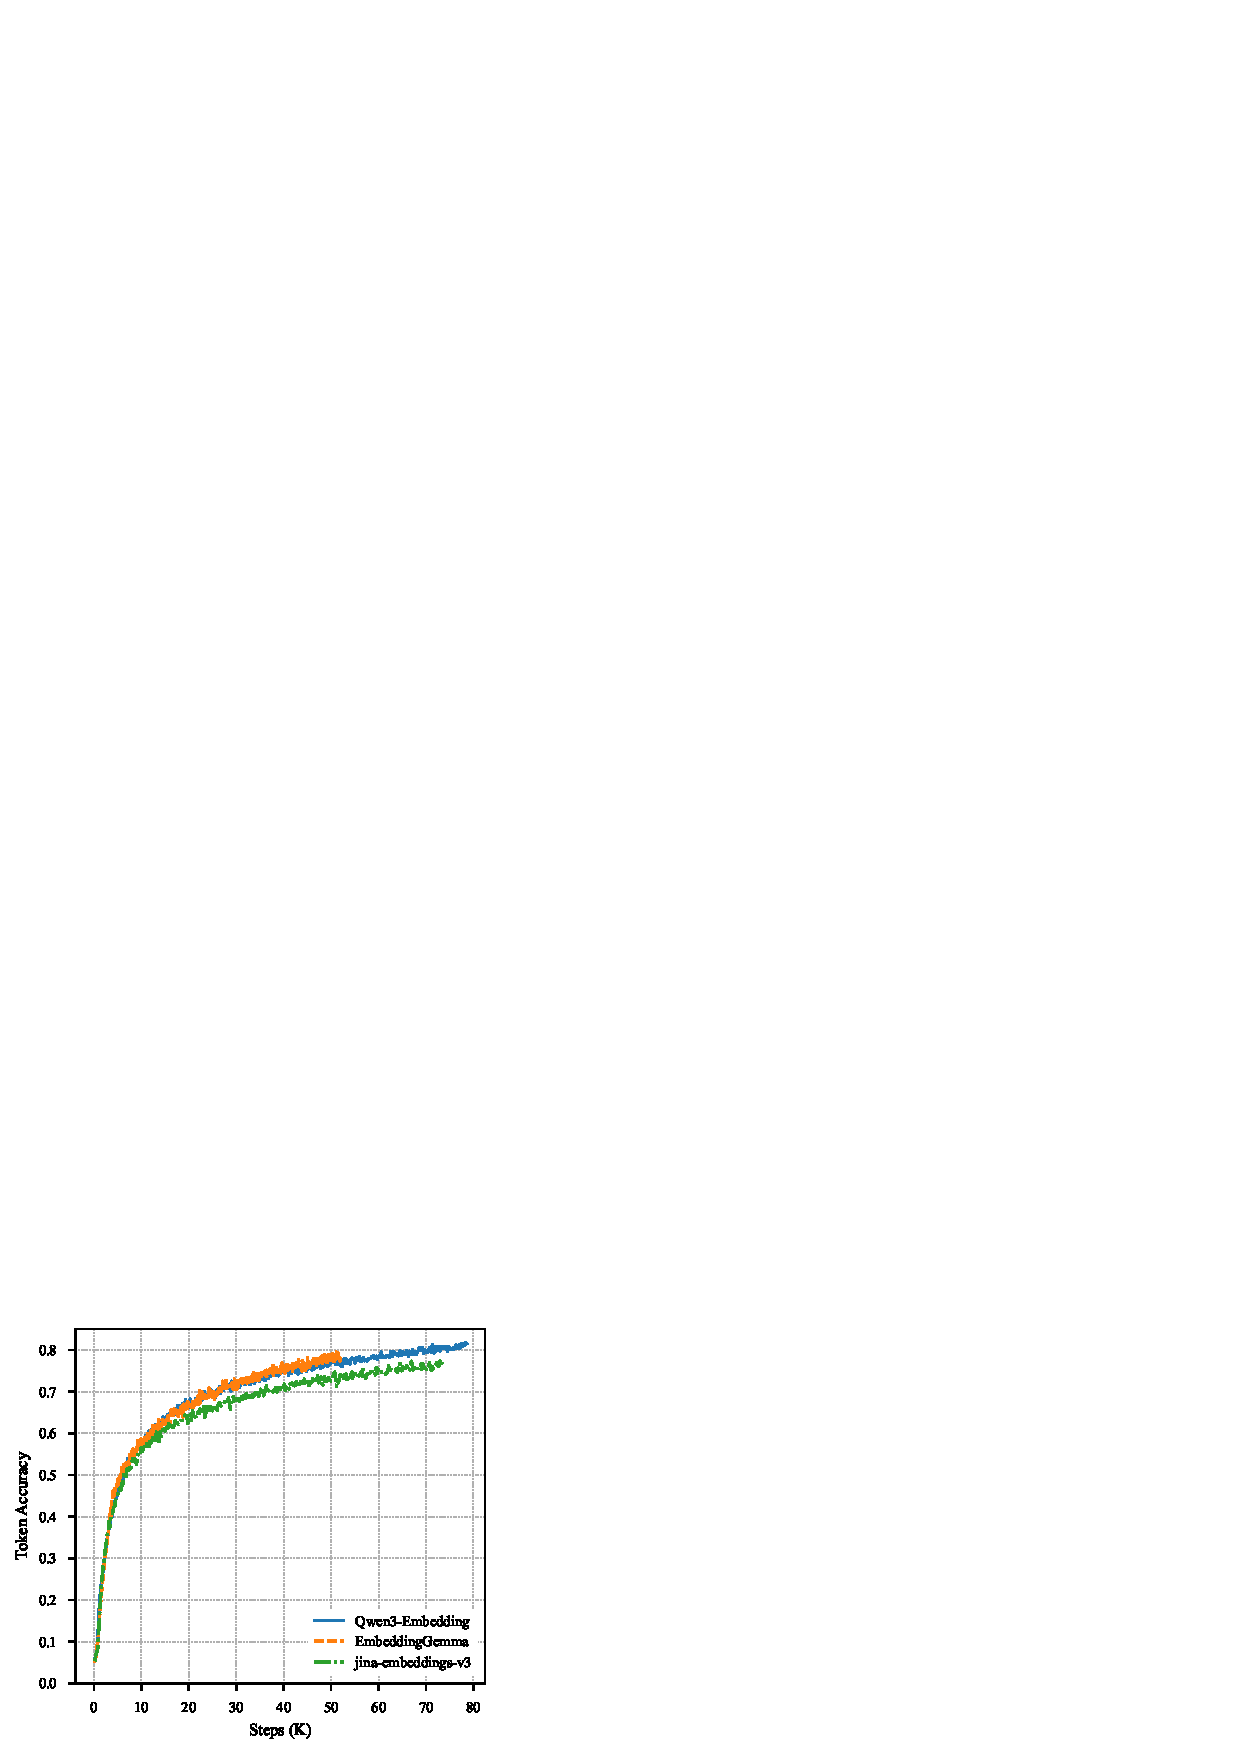
\includegraphics[width=\textwidth]{figures/acc-curves.pdf}
\caption{Token accuracy}
\end{subfigure}
\hfill
\begin{subfigure}[t]{0.49\textwidth}
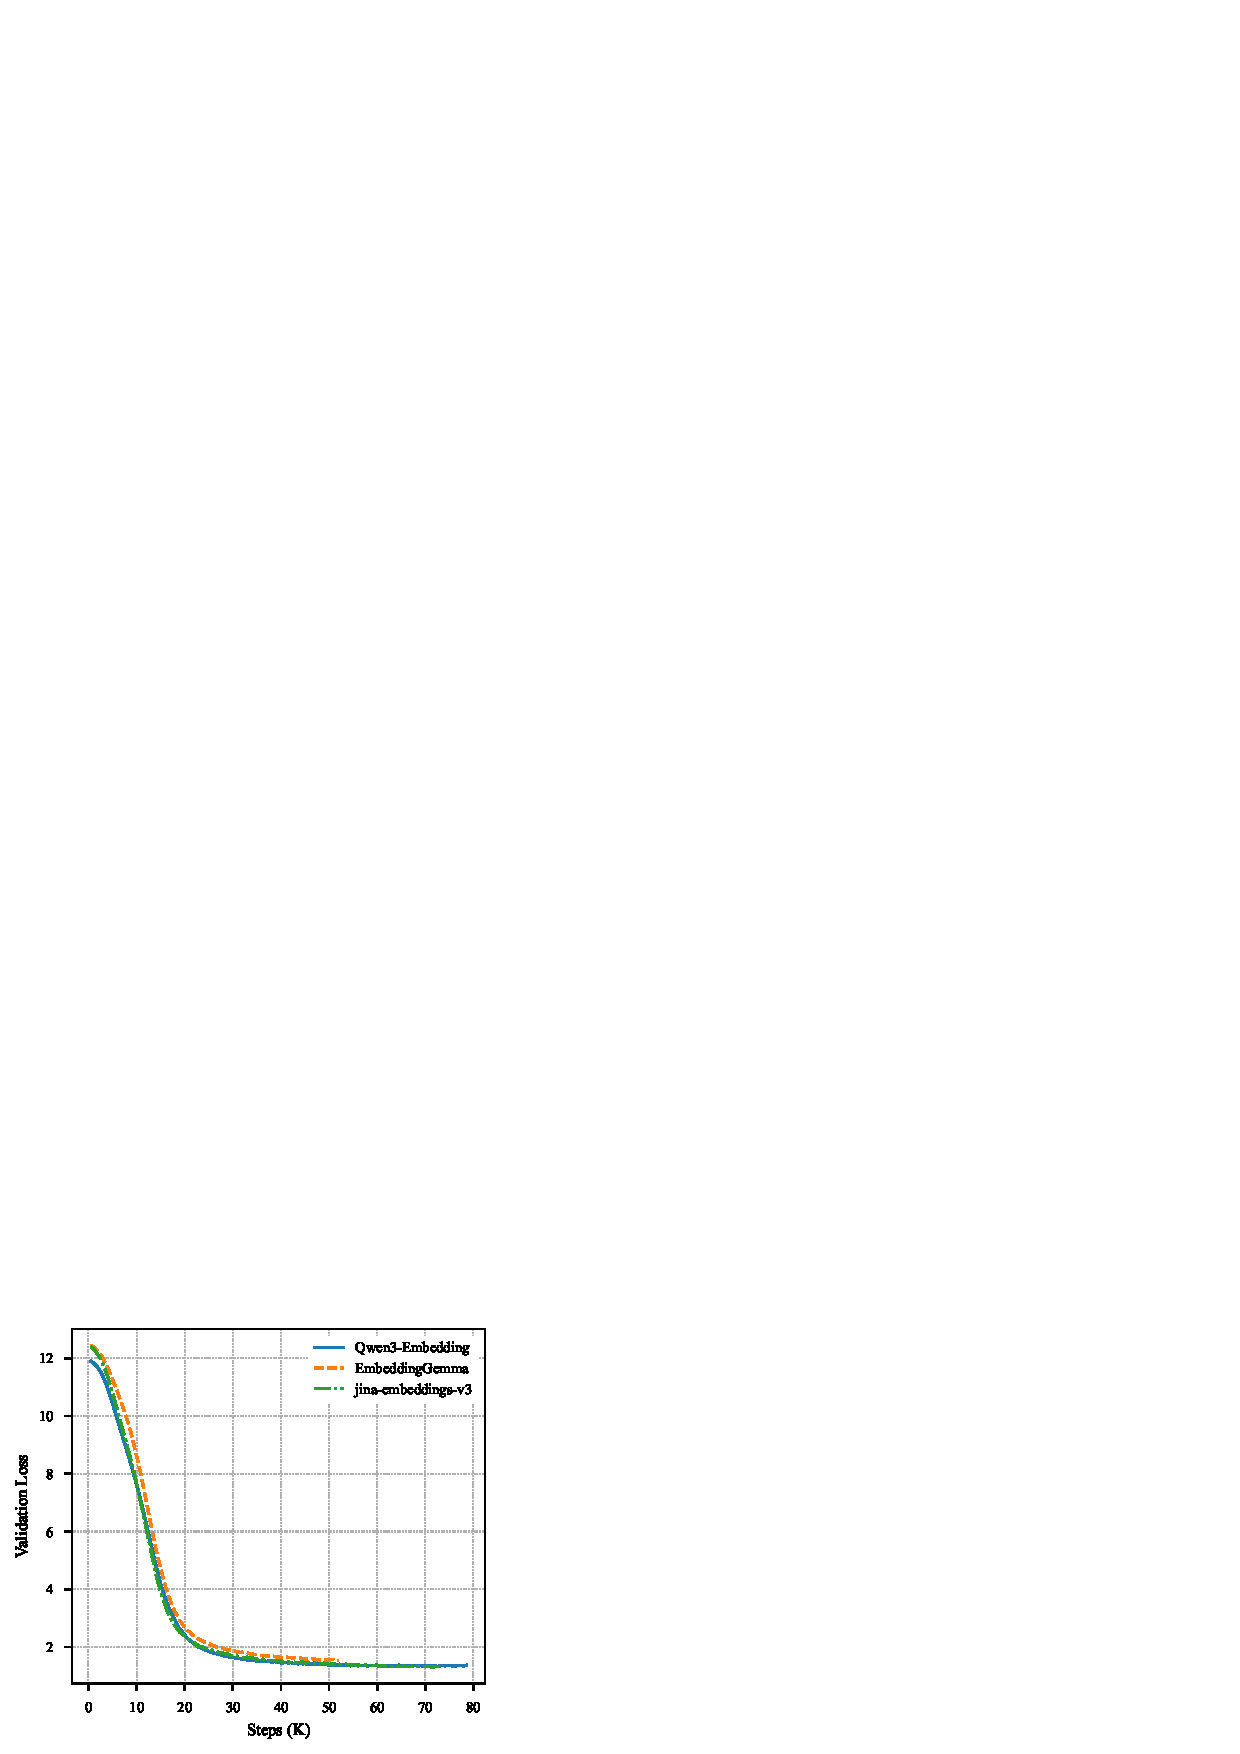
\includegraphics[width=\textwidth]{figures/valloss-curves.pdf}
\caption{Validation loss}
\end{subfigure}
\caption{Training dynamics across three embedding encoders on 2M multilingual samples. Qwen3-Embedding reaches 81.3\% token accuracy at 72.5K steps with validation loss 1.32. All models show diminishing returns beyond 50K steps, suggesting architectural improvements rather than extended training as the path to further gains.}
\label{fig:training-curves}
\end{figure}

\section{Conclusion}

We presented embedding inversion via conditional masked diffusion, achieving 81.3\% token accuracy across three embedding models with a 78M parameter decoder that requires no access to the target encoder. As inversion methods evolve from architecture specific to fully agnostic, embeddings should be treated as sensitive data requiring protection equivalent to the original text.

\bibliographystyle{plainnat}
\bibliography{references}

\appendix

\section{Implementation Details}

\subsection{Hyperparameters}

\begin{table}[h]
\centering
\caption{Complete hyperparameter configuration.}
\begin{tabular}{ll}
\toprule
Parameter & Value \\
\midrule
Transformer layers & 8 \\
Hidden dimension & 768 \\
Attention heads & 12 \\
MLP dimension & 3072 \\
Dropout & 0.1 \\
Batch size & 400 \\
Learning rate & $10^{-4}$ \\
Weight decay & 0.01 \\
EMA decay & 0.9999 \\
Noise schedule $\lambda$ & 5.0 \\
Sequence length & 32 \\
Training steps & 200K \\
\bottomrule
\end{tabular}
\end{table}

\subsection{Computational Requirements}

Training on a single A100 GPU takes approximately 48 hours for 200K steps. Inference using sequential decoding takes 150ms per sequence on the same hardware. Euler sampling is significantly faster at approximately 50ms per sequence due to parallel token prediction, though it achieves slightly lower quality. Memory requirements during training peak at 24GB including optimizer states and activations for the batch size of 400. The model checkpoint size is 312MB including both model parameters and EMA weights.

\begin{table}[h]
\centering
\caption{Performance milestones during training for jina-v3 encoder. Sequential greedy decoding.}
\label{tab:milestones}
\begin{tabular}{lcccc}
\toprule
Training Steps & Token Acc. & Exact Match & Cosine Sim. & BLEU \\
\midrule
10K & 40.2\% & 1.3\% & 0.65 & 22.1 \\
25K & 58.7\% & 5.8\% & 0.76 & 35.4 \\
50K & 69.7\% & 12.3\% & 0.83 & 45.2 \\
100K & 70.8\% & 13.7\% & 0.84 & 46.8 \\
200K & 71.2\% & 14.1\% & 0.84 & 47.3 \\
\bottomrule
\end{tabular}
\end{table}

\section{Qualitative Examples}

Tables~\ref{tab:qual-decode}--\ref{tab:qual-gemma} show qualitative inversion examples. Table~\ref{tab:qual-decode} compares four decoding strategies on the same English input using jina-embeddings-v3. Tables~\ref{tab:qual-jinav3}, \ref{tab:qual-qwen3}, and \ref{tab:qual-gemma} show sequential greedy decoding across six languages for each encoder.

\begin{table}[h]
\centering
\caption{Decoding strategy comparison on jina-embeddings-v3. Input: ``The advancement of artificial intelligence has fundamentally transformed modern society.''}
\label{tab:qual-decode}
\small
\begin{tabular}{p{0.22\linewidth}p{0.62\linewidth}c}
\toprule
Method & Recovered Text & Sim. \\
\midrule
Sequential & \scriptsize The revolution of artificial society is a new technology that is the most advanced in the world. The goal of the world is to increase the lives of the people & 0.82 \\
Euler & \scriptsize The imagination that we transformed and automitting technology has become optimized by the modern Intelligence Agency that the world has endured in revolutionary technologies that & 0.80 \\
Euler + Remask & \scriptsize Artificial is the future of the outbreak of mischievous technology. Many people around the world are analyzed by transforming society by life, of & 0.78 \\
Two-Stage & \scriptsize Today, the AI industry is one of the the sight revolutions, a history of Modern and Advanced Languages. He has brought the world of Artificial & 0.79 \\
\bottomrule
\end{tabular}
\end{table}

\begin{table}[h]
\centering
\caption{Multilingual inversion examples using jina-embeddings-v3 with sequential greedy decoding.}
\label{tab:qual-jinav3}
\small
\begin{tabular}{p{0.08\linewidth}p{0.40\linewidth}p{0.40\linewidth}c}
\toprule
Lang & Original & Recovered & Sim. \\
\midrule
en & \scriptsize The advancement of artificial intelligence has fundamentally transformed modern society. & \scriptsize The revolution of artificial society is a new technology that is the most advanced in the world. & 0.82 \\
zh & \scriptsize \zh{人工智能的进步从根本上改变了现代社会解决复杂问题的方式。} & \scriptsize The complexity of the modern life changes in complexity. The problem is that the problem is to create a new life in the world. & 0.65 \\
de & \scriptsize Die Fortschritte in der k\"{u}nstlichen Intelligenz haben die moderne Gesellschaft grundlegend ver\"{a}ndert. & \scriptsize The modern world of the modern society is increasingly changing in the world of the modern life. & 0.69 \\
ja & \scriptsize \ja{人工知能の進歩は現代社会における問題解決の方法を根本的に変革しました。} & \scriptsize The modern life changes in the world of the problem. The problem of the problem is to transform the complexity of the artificial intelligence. & 0.76 \\
fr & \scriptsize Les progr\`{e}s de l'intelligence artificielle ont fondamentalement transform\'{e} la soci\'{e}t\'{e} moderne. & \scriptsize The transformation of the modern society is the most important factor in the world. & 0.70 \\
es & \scriptsize Los avances en inteligencia artificial han transformado fundamentalmente la sociedad moderna. & \scriptsize The modern revolution of the artificial society is a major transformation in the United States. & 0.81 \\
\bottomrule
\end{tabular}
\end{table}

\begin{table}[h]
\centering
\caption{Multilingual inversion examples using Qwen3-Embedding with sequential greedy decoding.}
\label{tab:qual-qwen3}
\small
\begin{tabular}{p{0.08\linewidth}p{0.40\linewidth}p{0.40\linewidth}c}
\toprule
Lang & Original & Recovered & Sim. \\
\midrule
en & \scriptsize The advancement of artificial intelligence has fundamentally transformed modern society. & \scriptsize The most widely accepted and transformative of the natural and social media in the contemporary and technological aspects of the entire life. & 0.78 \\
zh & \scriptsize \zh{人工智能的进步从根本上改变了现代社会解决复杂问题的方式。} & \scriptsize The world has become more complex than ever before, as a result of the real problem of the way, the new ways of the artificial intelligence. & 0.65 \\
de & \scriptsize Die Fortschritte in der k\"{u}nstlichen Intelligenz haben die moderne Gesellschaft grundlegend ver\"{a}ndert. & \scriptsize The real-life of the German civilization is transforming the world into the technology of the German civilization. & 0.65 \\
ja & \scriptsize \ja{人工知能の進歩は現代社会における問題解決の方法を根本的に変革しました。} & \scriptsize The world of human society is increasingly important in the ways of the human society as the result of the new generation. & 0.57 \\
fr & \scriptsize Les progr\`{e}s de l'intelligence artificielle ont fondamentalement transform\'{e} la soci\'{e}t\'{e} moderne. & \scriptsize The real life of the society is the increase of the the chemical in the the et aux it\'{e} de la la de la de la. & 0.65 \\
es & \scriptsize Los avances en inteligencia artificial han transformado fundamentalmente la sociedad moderna. & \scriptsize The real world of the way the technology is transforming the average of the natural and social media in the entire world. & 0.67 \\
\bottomrule
\end{tabular}
\end{table}

\begin{table}[h]
\centering
\caption{Multilingual inversion examples using EmbeddingGemma with sequential greedy decoding.}
\label{tab:qual-gemma}
\small
\begin{tabular}{p{0.08\linewidth}p{0.40\linewidth}p{0.40\linewidth}c}
\toprule
Lang & Original & Recovered & Sim. \\
\midrule
en & \scriptsize The advancement of artificial intelligence has fundamentally transformed modern society. & \scriptsize The systems of the most important to the human intelligence, the most important to the human sector of the modern approach. & 0.68 \\
zh & \scriptsize \zh{人工智能的进步从根本上改变了现代社会解决复杂问题的方式。} & \scriptsize A complex system is a complex approach to the systems of the ability to develop the most powerful and the ability to develop. & 0.61 \\
de & \scriptsize Die Fortschritte in der k\"{u}nstlichen Intelligenz haben die moderne Gesellschaft grundlegend ver\"{a}ndert. & \scriptsize Die Forschung ist die Zeit der Zeit der Entwicklung von der Zeit der Entwicklung der Entwicklung der Zeit von der Welt. & 0.57 \\
ja & \scriptsize \ja{人工知能の進歩は現代社会における問題解決の方法を根本的に変革しました。} & \scriptsize A system of the systems of the human development of the importance of the current and the ability to develop the cell-based approach. & 0.59 \\
fr & \scriptsize Les progr\`{e}s de l'intelligence artificielle ont fondamentalement transform\'{e} la soci\'{e}t\'{e} moderne. & \scriptsize La technologie de la s\'{e}rie de la soci\'{e}t\'{e} de la plan\`{e}te, de la gestion de la plan\`{e}te, de la science. & 0.62 \\
es & \scriptsize Los avances en inteligencia artificial han transformado fundamentalmente la sociedad moderna. & \scriptsize La ingenier\'{i}a de la historia de la inteligencia de la organizaci\'{o}n de la atenci\'{o}n de la que las tecnolog\'{i}as. & 0.64 \\
\bottomrule
\end{tabular}
\end{table}

\end{document}
